\section{Specifica dei test}
\label{specificaDeiTest}
	\subsection{Descrizione dei test}
	\label{descrizioneDeiTest}
		Vengono ora indicati i test di validazione, di sistema e di integrazione previsti. I test di unità saranno inseriti in un momento successivo. \\
		Poiché i test saranno applicati in uno stadio di lavoro successivo a quello attuale, lo stato dei singoli è indicato come \textbf{N.I.}: non implementati. \\
		Di ogni test verranno indicati la tipologia ed altri parametri come specificato dalla seguente sintassi:
		\begin{itemize}
					\item per i test di unità: \textbf{TU[Codice Test]};
					\item per i test di integrazione: \textbf{TI[Identificativo del componente]};
					\item per i test di sistema: \textbf{TS[Tipo Requisito][Codice Requisito]};
					\item per i test di validazione: \textbf{TV[Tipo Requisito][Codice Requisito]}.
		\end{itemize}
		In particolare:
		\begin{itemize}
			\item \textbf{Codice Requisito}: è il codice gerarchico univoco di ogni vincolo espresso in numero (esempio: 1.3.2);
			\item \textbf{Identificativo del componente}: corrisponde al componente i cui elementi sono integrati;
			\item \textbf{Tipo Requisito}: può assumere solo uno fra i seguenti valori:
			\begin{itemize}
				\item F: funzionale;
				\item Q: di qualità;
				\item P: prestazionale;
				\item V: di vincolo.
			\end{itemize}
		\end{itemize}
	\subsection{Modello a V}
	\label{modelloAV}
			Per la specificazione dei test si utilizzerà il Modello a V. Secondo questo modello il testing del software viene suddiviso in livelli differenti, i quali si concretizzano in un'esecuzione bottom-up che avanza sequenzialmente alle attività di codifica e di validazione. Ad ogni livello corrisponde un ciclo di uno specifico tipo di test, ed ogni test viene creato in base al relativo livello di progettazione.
			\begin{figure}[htp]
				\centering
				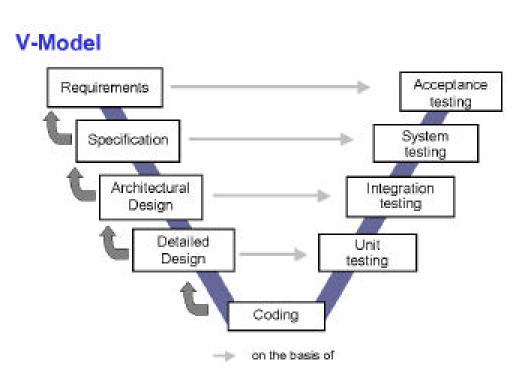
\includegraphics[width=0.5\textwidth]{img/V-model.jpg}
				\caption{Modello a V}
			\end{figure}
	\subsection{Test di validazione}
	\label{testDiValidazione}

I test di validazione servono per accertarsi che il prodotto realizzato sia conforme alle attese di \PROPONENTE. \\
Per ognuno vengono indicati i passi necessari all'utente per testare i requisiti associati. Il tracciamento tra i test di validazione e i requisiti correlati viene riportato nel documento \ARdoc.
\begin{tabella}{!{\VRule}l!{\VRule}X[l,b,l]!{\VRule}X[l,b,l]!{\VRule}}\intestazionethreecol{Test}{Descrizione}{Operazioni}TV0F1 & L'utente vuole verificare di poter possedere un account.
 & Viene richiesto di: \begin{enumerate} 
\item registrare un account; 
\item autenticarsi con i dati del proprio account. 
\end{enumerate} \\ 
TV0F1.1 & L'utente vuole verificare che si possa autenticare. & Viene richiesto di: \begin{enumerate} 
\item inserire un indirizzo email nel campo apposito; 
\item inserire una password nel campo apposito; 
\item confermare i dati inseriti; 
\item verificare di essere autenticato se i dati inseriti sono corretti; 
\item verificare se viene segnalato ogni eventuale errore durante la procedura di autenticazione. 
\end{enumerate} \\ 
TV0F1.1.1 & L'utente vuole verificare che l'autenticazione richieda l'inserimento di una mail. & Viene richiesto di: \begin{enumerate} 
\item non inserire alcuna mail; 
\item verificare che il sistema faccia visualizzare l'errore relativo. 
\end{enumerate} \\ 
TV0F1.1.2 & L'utente vuole verificare che l'autenticazione richieda una password. & Viene richiesto di: \begin{enumerate} 
\item non inserire alcuna password; 
\item verificare che il sistema faccia visualizzare l'errore relativo. 
\end{enumerate} \\ 
TV0F1.1.3 & L'utente vuole verificare che si possa confermare l'autenticazione. & Viene richiesto di: \begin{enumerate} 
\item cliccare sul pulsante di conferma; 
\item verificare che l'autenticazione avvenga correttamente se i dati sono corretti, altrimenti vengano mostrati gli errori. 
\end{enumerate} \\ 
TV0F1.1.4 & L'utente vuole verificare che se i dati sono corretti egli viene autenticato. & Viene richiesto di: \begin{enumerate} 
\item inserire i dati corretti richiesti dall'autenticazione; 
\item confermare i dati cliccando l'apposito pulsante; 
\item verificare di essere autenticato. 
\end{enumerate} \\ 
TV0F1.1.5 & L'utente vuole verificare che, ogni eventuale errore riguardante la procedura di autenticazione, interrompa la procedura stessa. & Viene richiesto di: \begin{enumerate} 
\item inserire i dati non corretti richiesti dall'autenticazione; 
\item confermare l'autenticazione cliccando l'apposito bottone; 
\item verificare che venga visualizzato il messaggio di errore di autenticazione. 
\end{enumerate} \\ 
TV0F1.1.5.1 & L'utente vuole verificare che il sistema interrompa l'autenticazione se la mail inserita non è presente nel sistema. & Viene richiesto di: \begin{enumerate} 
\item inserire una mail non presente nel database dell'applicazione; 
\item confermare l'autenticazione cliccando l'apposito bottone; 
\item verificare che venga mostrato l'errore di autenticazione. 
\end{enumerate} \\ 
TV0F1.1.5.2 & L'utente vuole verificare che il sistema interrompa l'autenticazione se la password inserita non coincide con quella associata alla mail. & Viene richiesto di: \begin{enumerate} 
\item inserire una mail valida; 
\item inserire una password errata; 
\item confermare l'autenticazione cliccando l'apposito tasto; 
\item verificare che venga mostrato l'errore di autenticazione. 
\end{enumerate} \\ 
TV0F1.1.5.3 & L'utente vuole verificare che il sistema mostri l'errore di autenticazione. & Viene richiesto di: \begin{enumerate} 
\item inserire i dati errati richiesti dall'autenticazione; 
\item confermare cliccando l'apposito bottone; 
\item verificare che venga visualizzato l'errore di autenticazione. 
\end{enumerate} \\ 
TV0F1.1.5.4 & L'utente vuole verificare di poter cambiare la password nel caso non se la ricordasse. & Viene richiesto di: \begin{enumerate} 
\item inserire l'indirizzo email con cui si è registrato; 
\item verificare di aver ricevuto un'email all'indirizzo inserito con una nuova password casuale; 
\item verificare che la vecchia password del proprio account venga sostituita con quella nuova inviata per email. 
\end{enumerate} \\ 
TV0F1.1.5.4.1 & L'utente vuole verificare che la richiesta di una nuova password richieda una mail. & Viene richiesto di: \begin{enumerate} 
\item non inserire una mail; 
\item confermare la richiesta di una nuova password cliccando l'apposito bottone; 
\item verificare che il sistema mostri l'errore di inserimento del dato. 
\end{enumerate} \\ 
TV0F1.1.5.4.2 & L'utente vuole verificare che la richiesta di una nuova password invii la nuova password al suo contatto mail. & Viene richiesto di: \begin{enumerate} 
\item completare la richiesta di una nuova password; 
\item verificare sulla propria casella di posta che sia stata inviata la nuova password. 
\end{enumerate} \\ 
TV0F1.1.5.4.3 & L'utente vuole verificare che il sistema abbia cambiato la password con la nuova password inviata. & Viene richiesto di: \begin{enumerate} 
\item effettuare l'autenticazione utilizzando la nuova password; 
\item verificare che l'autenticazione vada a buon fine. 
\end{enumerate} \\ 
TV0F1.1.5.4.4 & L'utente vuole verificare che il sistema interrompa la richiesta di nuova password se la mail inserita non è è presente nel database. & Viene richiesto di: \begin{enumerate} 
\item non inserire la mail corretta; 
\item confermare la richiesta di nuova password cliccando l'apposito bottone; 
\item verificare che il sistema interrompa la procedura mostrando l'errore apposito. 
\end{enumerate} \\ 
TV0F1.1.5.4.5 & L'utente vuole verificare che il sistema segnali l'errore di mail non presente nel database. & Viene richiesto di: \begin{enumerate} 
\item inserire una mail non presente nel database; 
\item confermare la richiesta di nuova password cliccando l'apposito bottone; 
\item verificare che venga visualizzato l'errore di mail non presente. 
\end{enumerate} \\ 
TV0F1.2 & L'utente vuole verificare di poter registrare un nuovo account. & Viene richiesto di: \begin{enumerate} 
\item inserire il proprio indirizzo email nell'apposito campo; 
\item inserire uno username nell'apposito campo; 
\item inserire una password nell'apposito campo; 
\item reinserire la password nell'apposito campo; 
\item confermare i dati inseriti cliccando l'apposito bottone; 
\item verificare che l'account venga registrato con i dati inseriti, se non ci sono stati errori, e che venga autenticato automaticamente. 
\end{enumerate} \\ 
TV0F1.2.1 & L'utente vuole verificare che la registrazione richieda la mail. & Viene richiesto di: \begin{enumerate} 
\item non inserire alcuna mail; 
\item confermare la registrazione cliccando l'apposito bottone; 
\item verificare che la registrazione mostri l'errore di mail mancante. 
\end{enumerate} \\ 
TV0F1.2.2 & L'utente vuole verificare che la registrazione richieda un username. & Viene richiesto di: \begin{enumerate} 
\item non inserire alcun username; 
\item confermare la registrazione cliccando l'apposito bottone; 
\item verificare che la registrazione mostri l'errore di username mancante. 
\end{enumerate} \\ 
TV0F1.2.3 & L'utente vuole verificare che la registrazione richieda la password. & Viene richiesto di: \begin{enumerate} 
\item non inserire alcuna password; 
\item confermare la registrazione cliccando l'apposito bottone; 
\item verificare che la registrazione mostri l'errore di password mancante. 
\end{enumerate} \\ 
TV0F1.2.4 & L'utente vuole verificare che la registrazione richieda di reinserire la password. & Viene richiesto di: \begin{enumerate} 
\item non reinserire la password; 
\item confermare la registrazione cliccando l'apposito bottone; 
\item verificare che la registrazione mostri l'errore di reinserimento della password errato. 
\end{enumerate} \\ 
TV0F1.2.5 & L'utente vuole verificare che la registrazione debba essere confermata tramite l'apposito bottone. & Viene richiesto di: \begin{enumerate} 
\item completare i campi richiesti dalla registrazione; 
\item confermare la registrazione cliccando l'apposito bottone; 
\item verificare che, se i dati sono corretti, si venga registrati, altrimenti vengano mostrati gli errori relativi ai dati. 
\end{enumerate} \\ 
TV0F1.2.6 & L'utente vuole verificare che se i dati inseriti sono corretti e si conferma la registrazione, egli viene registrato. & Viene richiesto di: \begin{enumerate} 
\item inserire tutti i dati richiesti dalla registrazione in modo corretto; 
\item confermare la registrazione cliccando l'apposito bottone; 
\item verificare che la registrazione vada a buon fine. 
\end{enumerate} \\ 
TV0F1.2.6.1 & L'utente vuole verificare che se la registrazione va a buon fine, egli viene automaticamente autenticato. & Viene richiesto di: \begin{enumerate} 
\item inserire i dati richiesti in modo corretto; 
\item confermare la registrazione cliccando l'apposito bottone; 
\item verificare di essere autenticati non appena la registrazione conclude con esito positivo. 
\end{enumerate} \\ 
TV0F1.2.7 & L’utente vuole verificare che il sistema avvisi l’utente che si sta registrando, che durante la procedura di registrazione è avvenuto un errore. & Viene richiesto di: \begin{enumerate} 
\item completare i campi richiesti dalla registrazione; 
\item confermare la registrazione cliccando l'apposito bottone; 
\item verificare che sia mostrato un avviso qualora ci siano stati errori. 
\end{enumerate} \\ 
TV0F1.2.7.1.1 & L'utente vuole verificare che una mail valida sia formata dal simbolo '@' preceduto da caratteri e seguita da un dominio valido. & Viene richiesto di: \begin{enumerate} 
\item inserire una mail che non rispetti i criteri per essere valida; 
\item confermare la registrazione cliccando l'apposito bottone; 
\item verificare che la registrazione venga interrotta e venga mostrato l'errore di mail non valida. 
\end{enumerate} \\ 
TV0F1.2.7.1.2 & L'utente vuole verificare che la mail inserita non debba essere già in uso. & Viene richiesto di: \begin{enumerate} 
\item inserire una mail già in uso; 
\item confermare la registrazione cliccando l'apposito bottone; 
\item verificare che la registrazione venga interrotta e venga mostrato l'errore di mail già in uso. 
\end{enumerate} \\ 
TV0F1.2.7.2 & L'utente vuole verificare che l'username richiesto debba essere valido. & Viene richiesto di: \begin{enumerate} 
\item inserire una un username non valido; 
\item confermare la registrazione cliccando l'apposito bottone; 
\item verificare che la registrazione venga interrotta e sia mostrato l'avviso di username non valido. 
\end{enumerate} \\ 
TV0F1.2.7.2.1 & L'utente vuole verificare che un username valido sia formato da solo caratteri alfanumerici. & Viene richiesto di: \begin{enumerate} 
\item inserire un username che non rispetti i criteri per essere valido; 
\item confermare la registrazione cliccando l'apposito bottone; 
\item verificare che la registrazione venga interrotta e venga mostrato l'errore di username non valido. 
\end{enumerate} \\ 
TV0F1.2.7.2.2 & L'utente vuole verificare che l'username inserito non debba essere già in uso. & Viene richiesto di: \begin{enumerate} 
\item inserire un'username già in uso; 
\item confermare la registrazione cliccando l'apposito bottone; 
\item verificare che la registrazione venga interrotta e venga mostrato l'errore di username già in uso. 
\end{enumerate} \\ 
TV0F1.2.7.3 & L'utente vuole verificare che la password deve avere un minimo di 6 caratteri e un massimo di 16. & Viene richiesto di: \begin{enumerate} 
\item inserire una password più corta o più lunga di quello stabilito; 
\item confermare la registrazione cliccando l'apposito bottone; 
\item verificare che la registrazione venga interrotta e venga mostrato l'errore di password non valida. 
\end{enumerate} \\ 
TV0F1.2.7.4 & L'utente vuole verificare che la password reinserita debba essere uguale a quella precedentemente inserita. & Viene richiesto di: \begin{enumerate} 
\item reinserire una password diversa da quella precedentemente inserita; 
\item confermare la registrazione cliccando l'apposito bottone; 
\item verificare che la registrazione venga interrotta e venga mostrato l'errore di password reinserita non coincidente. 
\end{enumerate} \\ 
TV0F2 & L'utente vuole verificare di poter fare il logout. & Viene richiesto di: \begin{enumerate} 
\item cliccare il bottone per effettuare il logout; 
\item verificare che sia stato effettuato il logout. 
\end{enumerate} \\ 
TV0F3 & L'utente vuole verificare di poter effettuare un percorso se si trova in un luogo con dei percorsi disponibili. & Viene richiesto di: \begin{enumerate} 
\item trovarsi in un luogo con dei percorsi disponibili; 
\item cliccare sul bottone per iniziare il percorso; 
\item verificare di poter svolgere il percorso seguendo le indicazioni. 
\end{enumerate} \\ 
TV0F3.1 & L'utente vuole verificare di poter giocare il percorso fino alla sua conclusione. & Viene richiesto di: \begin{enumerate} 
\item iniziare il percorso cliccando sul bottone di inizio percorso; 
\item svolgere il percorso seguendo le indicazioni; 
\item verificare di poter svolgere il percorso fino alla sua conclusione. 
\end{enumerate} \\ 
TV0F3.1.1 & L'utente vuole verificare di poter cercare e trovare il beacon della prima stazione. & Viene richiesto di: \begin{enumerate} 
\item muoversi all'interno dell'edificio per cercare il beacon della prima stazione; 
\item verificare che sia possibile cercare il beacon della prima stazione; 
\item verificare che, se si è nei paraggi del beacon della prima stazione, si possa trovarlo. 
\end{enumerate} \\ 
TV0F3.1.1.1 & L'utente vuole verificare che se il dispositivo trova il beacon della stazione ricercata egli può iniziare agiocare la prova. & Viene richiesto di: \begin{enumerate} 
\item recarsi al beacon della stazione che sta cercando; 
\item verificare di poter iniziare a giocare la prova della stazione cliccando l'apposito bottone di inizio prova. 
\end{enumerate} \\ 
TV0F3.1.1.2 & L'utente vuole verificare che il dispositivo ignori i beacon che non sono quello che si sta cercando. & Viene richiesto di: \begin{enumerate} 
\item recarsi presso un beacon che non sia quello che si sta cercando; 
\item verificare che il dispositivo ignori il beacon. 
\end{enumerate} \\ 
TV0F3.1.2 & L'utente vuole verificare di poter svolgere la prova della stazione in cui si trova. & Viene richiesto di: \begin{enumerate} 
\item trovarsi nella stazione giusta; 
\item verificare di poter iniziare  e concludere di giocare la prova della stazione in cui si trova. 
\end{enumerate} \\ 
TV0F3.1.2.1 & L'utente vuole verificare che la prova che viene proposta sia una di quelle previste. & Viene richiesto di: \begin{enumerate} 
\item trovarsi nella stazione esatta; 
\item iniziare la prova della stazione cliccando il bottone di inizio prova; 
\item verificare che il sistema somministri una prova corretta. 
\end{enumerate} \\ 
TV0F3.1.2.2 & L'utente vuole verificare che gli vengano mostrate le istruzioni per lo svolgimento della prova. & Viene richiesto di: \begin{enumerate} 
\item trovarsi nella stazione corretta; 
\item verificare che vengano mostrate le istruzioni per lo svolgimento della prova. 
\end{enumerate} \\ 
TV0F3.1.2.3 & L'utente vuole verificare di poter giocare la prova. & Viene richiesto di: \begin{enumerate} 
\item iniziare la prova cliccando sul bottone di inizio prova; 
\item verificare di poter giocare la prova fino alla sua conclusione. 
\end{enumerate} \\ 
TV0F3.1.2.4 & L'utente vuole verificare che al termine della prova venga mostrato il risultato ottenuto. & Viene richiesto di: \begin{enumerate} 
\item giocare la prova fino alla sua conclusione; 
\item verificare che una volta conclusa la prova venga mostrato il risultato ottenuto. 
\end{enumerate} \\ 
TV0F3.1.2.5 & L'utente vuole verificare che una volta conclusa la prova sia possibile continuare con lo svolgimento del percorso. & Viene richiesto di: \begin{enumerate} 
\item giocare la prova fino alla sua conclusione; 
\item verificare di poter continuare lo svolgimento del percorso una volta conclusa la prova. 
\end{enumerate} \\ 
TV0F3.1.2.5.1 & l'utente vuole verificare che, se la prova non è l'ultima del percorso, vengono mostrate le istruzioni per trovare la prossima stazione. & Viene richiesto di: \begin{enumerate} 
\item concludere una prova che non sia l'ultima del percorso; 
\item verificare che vengano mostrate le istruzioni per trovare la prossima stazione. 
\end{enumerate} \\ 
TV0F3.1.2.5.1.1 & L'utente vuole verificare che una volta conclusa la prova della stazione in cui si trova, vengano mostrate le istruzioni per trovare la stazione seguente. & Viene richiesto di: \begin{enumerate} 
\item giocare la prova fino alla sua conclusione; 
\item verificare che vengano mostrate le istruzioni per la ricerca della nuova stazione. 
\end{enumerate} \\ 
TV0F3.1.2.5.2 & L'utente vuole verificare che se la prova è l'ultima del percorso egli ha concluso il percorso. & Viene richiesto di: \begin{enumerate} 
\item completare tutte le prove; 
\item verificare che una volta finita l'ultima prova sia abbia concluso anche il percorso. 
\end{enumerate} \\ 
TV0F3.2 & L'utente vuole verificare di poter visualizzare correttamente i risultati del percorso ottenuti una volta che ha concluso tutte le prove. & Viene richiesto di: \begin{enumerate} 
\item concludere tutte le prove; 
\item verificare che vengano mostrati i risultati ottenuti nel percorso. 
\end{enumerate} \\ 
TV0F3.2.1 & L'utente vuole verificare che, una volta concluso il percorso, venga mostrato il tempo totale che egli ci ha messo a   completarlo. & Viene richiesto di: \begin{enumerate} 
\item concludere tutte le prove; 
\item verificare che venga mostrato il tempo totale per completare il percorso. 
\end{enumerate} \\ 
TV0F3.2.1.1 & L'utente vuole verificare che il tempo totale venga calcolato dal momento in cui si accetta di giocare il percorso a quando si conclude l'ultima prova.
 & Viene richiesto di: \begin{enumerate} 
\item annotarsi l'ora di inizio dello svolgimento del percorso; 
\item concludere tutte le prove del percorso; 
\item annotarsi l'ora di conclusione del percorso; 
\item verificare che il tempo mostrato dall'applicazione sia uguale al tempo calcolato con le rilevazioni fatte.
\end{enumerate} \\ 
TV0F3.2.2 & L'utente vuole verificare che, una volta concluso il percorso, venga mostrato il tempo totale che egli ha impiegato per completare tutte le prove.
 & Viene richiesto di: \begin{enumerate} 
\item completare tutte le prove; 
\item verificare che venga mostrato il tempo totale per completare tutte le prove.
\end{enumerate} \\ 
TV0F3.2.2.1 & L'utente vuole verificare che il tempo totale per svolgere tutte le prove sia calcolato sommando i tempi per concludere le varie prove (senza quindi contare il tempo per gli spostamenti da stazione a stazione).
 & Viene richiesto di: \begin{enumerate} 
\item completare le varie prove annotandosi i tempi per svolgerle; 
\item verificare che il tempo mostrato sia la somma dei tempi per svolgere le varie prove.
\end{enumerate} \\ 
TV0F3.2.2.1.1 & L'utente vuole verificare che il tempo per svolgere una prova sia calcolato dal momento in cui si accetta di affrontarla a quando la si conclude.
All'utente viene richiesto di: & Viene richiesto di: \begin{enumerate} 
\item annotare il tempo di inizio della prova; 
\item annotare il tempo di conclusione della prova; 
\item verificare che il tempo venga calcolato dal tempo trascorso dall'inizio alla fine della prova.
\end{enumerate} \\ 
TV0F3.2.3 & L'utente vuole verificare che venga mostrato il punteggio totale una volta concluso il percorso. & Viene richiesto di: \begin{enumerate} 
\item concludere tutte le prove; 
\item verificare che venga mostrato il punteggio totale del percorso. 
\end{enumerate} \\ 
TV0F3.2.3.1 & L'utente vuole verificare che il punteggio totale venga calcolato sommando i punteggi delle prove. & Viene richiesto di: \begin{enumerate} 
\item concludere tutte le prove e annotare i punteggi delle prove; 
\item verificare che il punteggio totale sia dato dalla somma dei punteggi di tutte le prove. 
\end{enumerate} \\ 
TV0F3.2.4 & L'utente vuole verificare che venga mostrata la posizione in classifica con il relativo punteggio. & Viene richiesto di: \begin{enumerate} 
\item concludere tutte le prove del percorso;
\item verificare che venga mostrata la posizione in classifica con il relativo punteggio.
\end{e numerate} \\ 
TV0F3.2.4.1 & L'utente vuole verificare di poter visualizzare la classifica generale. & Viene richiesto di: \begin{enumerate} 
\item concludere tutte le prove del percorso; 
\item verificare di poter visualizzare la classifica generale. 
\end{enumerate} \\ 
TV0F3.2.5 & L'utente vuole verificare che venga mostrata la prova in cui ha ottenuto il punteggio più alto. & Viene richiesto di: \begin{enumerate} 
\item concludere tutte le prove del percorso; 
\item verificare che venga mostrata la prova in cui ha ottenuto il miglior punteggio. 
\end{enumerate} \\ 
TV0F3.2.6 & L'utente vuole verificare che venga mostrata la prova in cui ha ottenuto il punteggio più basso. & Viene richiesto di: \begin{enumerate} 
\item concludere tutte le prove del percorso; 
\item verificare che venga mostrata la prova in cui ha ottenuto il peggior punteggio. 
\end{enumerate} \\ 
TV0F3.3 & L'utente vuole verificare che, se è autenticato, può salvare i risultati del percorso. & Viene richiesto di: \begin{enumerate} 
\item concludere tutte le prove del percorso; 
\item verificare di poter salvare i risultati del percorso, cliccando sull'apposito bottone, se già autenticato. 
\end{enumerate} \\ 
TV0F4 & L'utente vuole verificare di poter visualizzare le informazioni relative all'app. & Viene richiesto di: \begin{enumerate} 
\item cliccare sulla sezione riguardante le informazioni relative all'app tramite l'apposito bottone; 
\item verificare di poter visualizzare le informazioni. 
\end{enumerate} \\ 
TV0F4.1 & L'utente vuole verificare che venga mostrata una descrizione generale dell'app. & Viene richiesto di: \begin{enumerate} 
\item accedere alla sezione riguardante le informazioni relative all'app tramite l'apposito bottone; 
\item verificare che venga visualizzata una descrizione generale dell'app. 
\end{enumerate} \\ 
TV0F4.2 & L'utente vuole verificare di poter accedere alla pagina web relativa all'app tramite un link. & Viene richiesto di: \begin{enumerate} 
\item accedere alla sezione riguardante le informazioni relative all'app tramite l'apposito bottone; 
\item verificare che sia presente un link alla pagina web relativa all'app e questa si apra tramite il browser predefinito del dispositivo. 
\end{enumerate} \\ 
TV0F4.3 & L'utente vuole verificare di poter inviare una segnalazione di errore tramite mail. & Viene richiesto di: \begin{enumerate} 
\item accedere alla sezione riguardante le informazioni relative all'app tramite l'apposito bottone; 
\item verificare che sia presente l'indirizzo mail per la segnalazione di errori. 
\end{enumerate} \\ 
TV0F4.3.1 & L'utente vuole verificare che, cliccando sull'indirizzo mail per la segnalazione di errori, venga aperto il gestore delle mail predefinito del dispositivo e che il destinatario sia quello su cui a cliccato. & Viene richiesto di: \begin{enumerate} 
\item accedere alla sezione riguardante le informazioni relative all'app tramite l'apposito bottone; 
\item cliccare sull'indirizzo mail per la segnalazione degli errori; 
\item verificare che si apra il gestore delle mail predefinito nel dispositivo e che il destinatario sia effettivamente quello per le segnalazioni d'errore. 
\end{enumerate} \\ 
TV0F5 & L'utente vuole verificare di poter visualizzare i risultati dei percorsi effettuati precedentemente. & Viene richiesto di: \begin{enumerate} 
\item accedere alla sezione riguardante i risultati dei percorsi tramite l'apposito bottone; 
\item verificare di poter visualizzare i risultati salvati qualora sia autenticato. 
\end{enumerate} \\ 
TV0F5.1 & L'utente vuole verificare di poter visualizzare la lista dei percorsi salvati qualora sia autenticato.
 & Viene richiesto di: \begin{enumerate} 
\item accedere alla sezione riguardante i risultati dei percorsi tramite l'apposito bottone; 
\item verificare che venga mostrata la lista dei suoi risultati salvati.
\end{enumerate} \\ 
TV0F5.1.1 & L'utente vuole verificare di poter visualizzare tutte le informazioni relative al percorso salvato scelto. & Viene richiesto di: \begin{enumerate} 
\item accedere alla sezione riguardante i risultati dei percorsi tramite l'apposito bottone; 
\item selezionare un risultato tra quelli salvati; 
\item verificare che vengano mostrate tutte le informazioni relative al percorso selezionato. 
\end{enumerate} \\ 
TV0F5.1.1.1 & L'utente vuole verificare che venga visualizzato il nome del percorso selezionato. & Viene richiesto di: \begin{enumerate} 
\item accedere alla sezione riguardante i risultati dei percorsi tramite l'apposito bottone; 
\item selezionare un risultato tra quelli salvati; 
\item verificare che venga visualizzato il nome del percorso. 
\end{enumerate} \\ 
TV0F5.1.1.2 & L'utente vuole verificare che venga visualizzato il nome del luogo dove è stato svolto il percorso selezionato. & Viene richiesto di: \begin{enumerate} 
\item accedere alla sezione riguardante i risultati dei percorsi tramite l'apposito bottone; 
\item selezionare un risultato tra quelli salvati; 
\item verificare che venga visualizzato il nome del luogo in cui è stato svolto il percorso. 
\end{enumerate} \\ 
TV0F5.1.1.3 & L'utente vuole verificare che venga visualizzata la data in cui si è svolto il percorso selezionato. & Viene richiesto di: \begin{enumerate} 
\item accedere alla sezione riguardante i risultati dei percorsi tramite l'apposito bottone; 
\item selezionare un risultato tra quelli salvati; 
\item verificare che venga visualizzata la data in cui è stato svolto il percorso. 
\end{enumerate} \\ 
TV0F5.1.1.4 & L'utente vuole verificare che venga visualizzato il punteggio totale ottenuto nel percorso selezionato. & Viene richiesto di: \begin{enumerate} 
\item accedere alla sezione riguardante i risultati dei percorsi tramite l'apposito bottone; 
\item selezionare un risultato tra quelli salvati; 
\item verificare che venga visualizzato il punteggio totale ottenuto nel percorso. 
\end{enumerate} \\ 
TV0F5.1.1.5 & L'utente vuole verificare che venga visualizzato il tempo totale impiegato per svolgere il percorso selezionato. & Viene richiesto di: \begin{enumerate} 
\item accedere alla sezione riguardante i risultati dei percorsi tramite l'apposito bottone; 
\item selezionare un risultato tra quelli salvati; 
\item verificare che venga visualizzato il tempo totale impiegato per svolgere il percorso. 
\end{enumerate} \\ 
TV0F5.1.1.6 & L'utente vuole verificare che venga visualizzato la posizione in classifica del percorso selezionato. & Viene richiesto di: \begin{enumerate} 
\item accedere alla sezione riguardante i risultati dei percorsi tramite l'apposito bottone; 
\item selezionare un risultato tra quelli salvati; 
\item  verificare che venga visualizzato la posizione in classifica del percorso. 
\end{enumerate} \\ 
TV0F5.2 & L'utente vuole verificare che se è autenticato ma non ha ancora salvato percorsi venga visualizzato un avviso che inviti a svolgerne almeno uno. & Viene richiesto di: \begin{enumerate} 
\item accedere alla sezione riguardante i risultati dei percorsi tramite l'apposito bottone; 
\item verificare che venga visualizzato un avviso che solleciti a svolgere e salvare almeno un percorso. 
\end{enumerate} \\ 
TV0F5.3 & L'utente vuole verificare che se non è autenticato viene visualizzato un messaggio che invita ad autenticarsi. & Viene richiesto di: \begin{enumerate} 
\item non effettuare il login; 
\item accedere alla sezione riguardante i risultati dei percorsi tramite l'apposito bottone; 
\item verificare che venga visualizzato un avviso che inviti ad autenticarsi. 
\end{enumerate} \\ 
TV0F6 & L'utente vuole verificare di poter visualizzare gli edifici con dei percorsi disponibili più vicini alla sua posizione. & Viene richiesto di: \begin{enumerate} 
\item accedere alla sezione riguardante la ricerca degli edifici tramite l'apposito bottone; 
\item verificare di poter visualizzare gli edifici con percorsi più vicini. 
\end{enumerate} \\ 
TV0F6.1.1 & L'utente vuole verificare di poter inserire un raggio in chilometri per la ricerca degli edifici. & Viene richiesto di: \begin{enumerate} 
\item accedere alla sezione riguardante la ricerca degli edifici tramite l'apposito bottone; 
\item verificare di poter inserire un raggio per la ricerca in chilometri. 
\end{enumerate} \\ 
TV0F6.1.1.1 & L'utente vuole verificare che se la ricerca tramite raggio va a buon fine vengano visualizzati gli edifici entro quel raggio. & Viene richiesto di: \begin{enumerate} 
\item accedere alla sezione riguardante la ricerca degli edifici tramite l'apposito bottone; 
\item inserire un raggio nel quale sia presente un edificio con percorsi; 
\item verificare che venga visualizzato l'edificio. 
\end{enumerate} \\ 
TV0F6.2 & L'utente vuole verificare di poter visualizzare tutte le informazioni relative all'edificio scelto tra la lista di ricerca degli edifici. & Viene richiesto di: \begin{enumerate} 
\item accedere alla sezione riguardante la ricerca degli edifici tramite l'apposito bottone; 
\item selezionare un edificio tra quelli nella lista; 
\item verificare che vengano visualizzate le informazioni relative a quell'edificio. 
\end{enumerate} \\ 
TV0F6.2.1 & L'utente vuole verificare di poter visualizzare tutte le informazioni specifiche dell'edificio.
 & Viene richiesto di: \begin{enumerate} 
\item accedere alla sezione riguardante la ricerca degli edifici tramite l'apposito bottone; 
\item selezionare un edificio tra quelli nella lista; 
\item verificare di poter visualizzare delle informazioni specifiche dell'edificio. 
\end{enumerate} \\ 
TV0F6.2.1.1 & L'utente vuole verificare che venga visualizzato il nome dell'edificio. & Viene richiesto di: \begin{enumerate} 
\item accedere alla sezione riguardante la ricerca degli edifici tramite l'apposito bottone; 
\item selezionare un edificio tra quelli della lista; 
\item verificare che venga visualizzato il nome dell'edificio. 
\end{enumerate} \\ 
TV0F6.2.1.2 & L'utente vuole verificare che venga visualizzata la destinazione d'uso dell'edificio. & Viene richiesto di: \begin{enumerate} 
\item accedere alla sezione riguardante la ricerca degli edifici tramite l'apposito bottone; 
\item selezionare un edificio tra quelli della lista; 
\item verificare che venga visualizzata la destinazione d'uso dell'edificio. 
\end{enumerate} \\ 
TV0F6.2.1.3 & L'utente vuole verificare che venga visualizzato l'indirizzo dell'edificio. & Viene richiesto di: \begin{enumerate} 
\item accedere alla sezione riguardante la ricerca degli edifici tramite l'apposito bottone; 
\item selezionare un edificio tra quelli della lista; 
\item verificare che venga visualizzato l'indirizzo dell'edificio. 
\end{enumerate} \\ 
TV0F6.2.2 & L'utente vuole verificare che venga visualizzato il link al sito web dell'edificio. & Viene richiesto di: \begin{enumerate} 
\item accedere alla sezione riguardante la ricerca degli edifici tramite l'apposito bottone; 
\item selezionare un edificio tra quelli della lista; 
\item verificare che venga visualizzato il link al sito web dell'edificio. 
\end{enumerate} \\ 
TV0F6.2.3 & L'utente vuole verificare di poter visualizzare tutti i contatti disponibili dell'edificio. & Viene richiesto di: \begin{enumerate} 
\item accedere alla sezione riguardante la ricerca degli edifici tramite l'apposito bottone; 
\item selezionare un edificio tra quelli della lista; 
\item verificare di poter visualizzare i contatti disponibili dell'edificio. 
\end{enumerate} \\ 
TV0F6.2.3.1 & L'utente vuole verificare di poter visualizzare il contatto telefonico dell'edificio. & Viene richiesto di: \begin{enumerate} 
\item accedere alla sezione riguardante la ricerca degli edifici tramite l'apposito bottone; 
\item selezionare un edificio tra quelli della lista; 
\item verificare di poter visualizzare il contatto telefonico dell'edificio. 
\end{enumerate} \\ 
TV0F6.2.3.2 & L'utente vuole verificare di poter visualizzare il contatto mail dell'edificio. & Viene richiesto di: \begin{enumerate} 
\item accedere alla sezione riguardante la ricerca degli edifici tramite l'apposito bottone; 
\item selezionare un edificio tra quelli della lista; 
\item verificare di poter visualizzare il contatto mail dell'edificio. 
\end{enumerate} \\ 
TV0F6.2.3.3 & L'utente vuole verificare di poter contattare contattare, tramite la pagina Facebook,  l'edificio, qualora sia disponibile. & Viene richiesto di: \begin{enumerate} 
\item accedere alla sezione riguardante la ricerca degli edifici tramite l'apposito bottone; 
\item selezionare un edificio tra quelli della lista; 
\item verificare, qualora sia disponibile, di poter contattare l'edificio tramite la pagina Facebook. 
\end{enumerate} \\ 
TV0F6.2.3.4 & L'utente vuole verificare di poter contattare contattare, tramite Twitter, l'edificio, qualora sia disponibile. & Viene richiesto di: \begin{enumerate} 
\item accedere alla sezione riguardante la ricerca degli edifici tramite l'apposito bottone; 
\item selezionare un edificio tra quelli della lista; 
\item verificare, qualora sia disponibile, di poter contattare l'edificio tramite Twitter. 
\end{enumerate} \\ 
TV0F6.2.3.5 & L'utente vuole verificare di poter contattare contattare, tramite contatto di WhatsApp, l'edificio, qualora sia disponibile. & Viene richiesto di: \begin{enumerate} 
\item accedere alla sezione riguardante la ricerca degli edifici tramite l'apposito bottone; 
\item selezionare un edificio tra quelli della lista; 
\item verificare, qualora sia disponibile, di poter contattare l'edificio tramite il contatto di WhatsApp. 
\end{enumerate} \\ 
TV0F6.2.3.6 & L'utente vuole verificare di poter contattare contattare, tramite contatto Telegram, l'edificio, qualora sia disponibile. & Viene richiesto di: \begin{enumerate} 
\item accedere alla sezione riguardante la ricerca degli edifici tramite l'apposito bottone; 
\item selezionare un edificio tra quelli della lista; 
\item verificare, qualora sia disponibile, di poter contattare l'edificio tramite il contatto di Telegram. 
\end{enumerate} \\ 
TV0F7 & L'utente verifica di poter cambiare le proprie credenziali d'accesso. & Viene richiesto di: \begin{enumerate} 
\item accedere al proprio profilo tramite l'apposito bottone; 
\item verificare di poter cambiare le proprie credenziali. 
\end{enumerate} \\ 
TV0F7.1 & L'utente vuole verificare di poter modificare il proprio username. & Viene richiesto di: \begin{enumerate} 
\item accedere al proprio profilo tramite l'apposito bottone; 
\item modificare il proprio username rispettando i requisiti R0F1.2.7.2.1 e R0F1.2.7.2.2; 
\item confermare il cambio delle credenziali cliccando l'apposito bottone; 
\item verificare di aver modificato il proprio username. 
\end{enumerate} \\ 
TV0F7.2 & L'utente vuole verificare di poter modificare la propria password. & Viene richiesto di: \begin{enumerate} 
\item accedere al proprio profilo tramite l'apposito bottone; 
\item modificare la propria password rispettando il requisito R0F1.2.7.3; 
\item confermare il cambio delle credenziali cliccando l'apposito bottone; 
\item verificare di aver modificato la propria password. 
\end{enumerate} \\ 
TV0F7.3 & L'utente vuole verificare che se i dati inseriti non sono corretti vengono visualizzati gli errori relativi. & Viene richiesto di: \begin{enumerate} 
\item accedere al proprio profilo tramite l'apposito bottone; 
\item modificare i propri dati con dati che non rispettano i requisiti R0F1.2.7.3, R0F1.2.7.2.1 e R0F1.2.7.2.2; 
\item confermare il cambio delle credenziali cliccando l'apposito bottone; 
\item verificare che venga interrotta la procedura di cambio credenziali e che vengano visualizzati gli errori relativi ai dati. 
\end{enumerate} \\ 
TV0Q1 & L'utente verifica se viene fornito il manuale per l'utente dell'applicazione. & Viene richiesto di: \begin{enumerate} 
\item verificare se viene fornito il manuale per l'utente dell'applicazione.
\end{enumerate} \\
\hiderowcolors
\caption{Riepilogo test di validazione}
\end{tabella}
		
	\subsection{Test di sistema}
	\label{testDiSistema}
		I test di sistema servono per accertarsi che il comportamento dinamico del sistema rispetti i requisiti software individuati e descritti nel documento \ARdoc.
		\subsubsection{Descrizione dei test di sistema}
			% tabella test di sistema esportati da trender
			\begin{tabella}{!{\VRule}l!{\VRule}X[l,b,l]!{\VRule}l!{\VRule}l!{\VRule}}
	\intestazionefourcol{Test}{Descrizione}{Stato}{Requisito}
TS0F1 & Viene verificato che il sistema permetta la creazione e la gestione di un account & N.I & \Req{R0F1} \\ 
TS0F2 & Viene verificato che il sistema permetta la deautenticazione dell'utente & N.I & \Req{R0F2} \\ 
TS0F3 & Viene verificato che il sistema permetta all'utente di giocare un percorso tra quelli disponibili nel luogo in cui si trova & N.I & \Req{R0F3} \\ 
TS0F4 & Viene verificato che il sistema permetta all'utente di visualizzare le informazioni dell'app & N.I & \Req{R0F4} \\ 
TS0F5 & Viene verificato che il sistema permetta all'utente di visualizzare i risultati dei percorsi effettuati precedentemente & N.I & \Req{R0F5} \\ 
TS0F6 & Viene verificato che il sistema permetta all'utente di cercare quali sono gli edifici con percorsi più vicini alla sua posizione & N.I & \Req{R0F6} \\ 
TS0F7 & Viene verificato che il sistema permetta all'utente di modificare le proprie credenziali d'accesso & N.I & \Req{R0F7} \\ 
TS0P1 & Viene verificato che in ogni schermata il tempo di latenza per ottenere una risposta dal server sia minore di 5 secondi, a meno che non vi siano problemi di connessione & N.I & \Req{R0P1} \\ 
TS0P2 & Viene verificato che il tempo di latenza per cambiare la schermata nell'app sia minore di 0.5 secondi, a meno che non sia richiesta l'interazione con il server & N.I & \Req{R0P2} \\ 
TS0Q1 & Viene verificato che il codice rispetti le norme e le metriche delle \NPdoc e della sezione \hyperref[metrichePerIlCodice]{Metriche per il codice} & N.I & \Req{R0Q1} \\ 
TS0Q2 & Viene verificato che i documenti rispettino le norme e le metriche delle \NPdoc e della \hyperref[metrichePerIlCodice]{Metriche per il codice} & N.I & \Req{R0Q2} \\ 
TS0Q3 & Viene verificato che venga fornito il manuale per l'utente & N.I & \Req{R0Q3} \\ 
TS2F8 & Viene verificato che il sistema permetta all'utente di visualizzare un tutorial introduttivo al primo utilizzo dell'app & N.I & \Req{R2F8} \\ 
\rowcolor{white}
\caption{Riepilogo test di sistema}
\end{tabella}
			
			
	\subsection{Test di integrazione}
	\label{testDiIntegrazione}
		I test di integrazione servono per verificare che tutti i diversi componenti del sistema comunichino correttamente tra loro, e che vi sia all'interno del software il flusso di dati atteso. \\
		Verrà utilizzata una strategia di integrazione incrementale per poter sviluppare e verificare più componenti in parallelo. Questo metodo permette di dare priorità ai test relativi alle componenti che vengono ritenute più importanti e quindi sarà possibile partire dalle componenti che soddisfano i requisiti obbligatori fino ad integrarle con quelle che soddisfano i requisiti opzionali. Inoltre permette di restringere la ricerca dell'errore in caso di test fallito, perché molto probabilmente l'errore si trova nel nuovo componente o dalla sua interazione con il sistema corrente. Non si dovrà escludere il caso in cui il test fallisca perché la nuova istanza di test utilizza un campione di input non trattato in precedenza, portando così il sistema a generare l'errore. \\
		L'integrazione delle parti è bottom-up: innanzitutto verranno inserite le componenti con meno dipendenze funzionali e più funzionalità, cioè che corrispondono ai requisiti obbligatori. Di conseguenza queste componenti saranno testate molte volte in modo da ridurre la possibilità che il prodotto finale contenga difetti, e così si otterrà una versione funzionante nel minor tempo possibile. In seguito si risalirà l'albero delle dipendenze fino all'inserimento delle componenti di alto livello. \\
		Questo metodo è più oneroso rispetto ad altri in quanto richiede che venga generato del codice di supporto, sotto forma di driver e stub, che simuli le componenti mancanti, però permette una maggiore copertura perché testa ripetutamente le componenti più importanti.
		
		
	\begin{tabella}{!{\VRule}l!{\VRule}X[l,b,l]!{\VRule}l}
		\intestazionetwocol{Test}{Descrizione}
		TIsavedresults & Verifica che il sistema gestisca correttamente la visualizzazione e il salvataggio dei risultati dei percorsi\\
		 TIdatamanager & Verifica che il sistema gestisca correttamente le richieste dei dati salvati in locale\\
		 TIpathprogress & Verifica che il sistema gestisca correttamente i dati del percorso selezionato e i risultati delle prove giocate\\
		  TIdataserver & Verifica che il sistema gestisca correttamente la modellazione dei dati locali del server \\
		  TIgames & Verifica che il sistema gestisca correttamente il percorso e le prove mentre si sta affrontando un percorso \\
		  TIserver & Verifica che il sistema gestisca correttamente la ricezione, l'elaborazione e la risposta alle richieste del client \\
		   TIlocation & Verifica che il sistema gestisca correttamente l'individuazione e la lettura dei beacon \\
		    TIclient & Verifica che il sistema gestisca ed integri correttamente tutte le parti del client, tra cui l'autenticazione, i percorsi e i servizi vari \\
		     TICLIPS & Verifica che il client e il server comunichino correttamente tra loro \\
		     TIauthentication & Verifica che il sistema gestisca correttamente la registrazione dell'account, il login e la modifica delle proprie credenziali\\ 
		     TIurlrequest & Verifica che il sistema gestisca correttamente le richieste da inviare la server\\
		     TIviewcontroller & Verifica che il sistema gestisca correttamente le pagine dell'applicazione e le risposte agli input dell'utente\\
		      TIutility & Verifica che il sistema gestisca correttamente le view generali dell'app\\
		       TIbuilding & Verifica che il sistema gestisca correttamente le view e le interazioni dell'utente riguardanti gli edifici abilitati e i relativi percorsi\\
		       TIurlrequesthandler & Verifica che il sistema gestisca correttamente le richieste del client e le risposte da inviare\\
		       TIdata & Verifica che il sistema gestisca correttamente la modellazione dei dati in locale\\
		       \end{tabella}


		\newpage
		\subsection{Test di unità}
		\label{testDiUnita}
		\begin{tabella}{!{\VRule}l!{\VRule}X[1,b,l]!{\VRule}l!{\VRule}c!{\VRule}}
	\intestazionefourcol{Test}{Descrizione}{Stato}{Esito}
	%I primi 24 test sono presi dalle chiamate del RequestMaker di urlrequest, del DataRequestMaker e del LoginManager di datamanager, i primi 12 sono relativi all'urlrequest e gli altri 12 invece a datamanager
	TU1 & Si verifica che la richiesta al server di ricevere i dati dell'applicazione restituisca, quando è corretta, la risposta giusta, o, quando è errata, l'errore corretto & IMPL. & {\color[rgb]{0.44,0.74,0.48} Superato}  \\
	TU2 & Si verifica che la richiesta al server di ricevere i risultati dei percorsi effettuati dall'utente restituisca, quando è corretta, la risposta giusta, o, quando è errata, l'errore corretto & IMPL. & {\color[rgb]{0.44,0.74,0.48} Superato}  \\
	TU3 & Si verifica che la richiesta al server di salvare i dati del percorso appena effettuato dall'utente restituisca, quando è corretta, la risposta giusta, o, quando è errata, l'errore corretto & IMPL. & {\color[rgb]{0.44,0.74,0.48} Superato}  \\
	TU4 & Si verifica che la richiesta al server di ricevere i dati del percorso selezionato dall'utente restituisca, quando è corretta, la risposta giusta, o, quando è errata, l'errore corretto & IMPL.  & {\color[rgb]{0.44,0.74,0.48} Superato} \\
	TU5 & Si verifica che la richiesta al server di ricevere i dati degli edifici più vicini all'utente restituisca, quando è corretta, la risposta giusta, o, quando è errata, l'errore corretto & IMPL. & {\color[rgb]{0.44,0.74,0.48} Superato}  \\
	TU6 & Si verifica che la richiesta al server di effettuare la registrazione del profilo dell'utente restituisca, quando è corretta, la risposta giusta, o, quando è errata, l'errore corretto & IMPL. & {\color[rgb]{0.44,0.74,0.48} Superato}  \\
	TU7 & Si verifica che la richiesta al server di effettuare il login dell'utente restituisca, quando è corretta, la risposta giusta, o, quando è errata, l'errore corretto & IMPL. & {\color[rgb]{0.44,0.74,0.48} Superato}  \\
	TU8 & Si verifica che la richiesta al server di effettuare il logout dell'utente restituisca, quando è corretta, la risposta giusta, o, quando è errata, l'errore corretto & IMPL. & {\color[rgb]{0.44,0.74,0.48} Superato} \\
	TU9 & Si verifica che la richiesta al server di effettuare la modifica dei dati del profilo dell'utente restituisca, quando è corretta, la risposta giusta, o, quando è errata, l'errore corretto & IMPL.& {\color[rgb]{0.44,0.74,0.48} Superato}  \\
	TU10 & Si verifica che la richiesta al server di effettuare il controllo sui dati inseriti dall'utente restituisca, quando è corretta, la risposta giusta, o, quando è errata, l'errore corretto & IMPL.& {\color[rgb]{0.44,0.74,0.48} Superato}  \\
	TU11 & Si verifica che la richiesta al server di ricevere i dati del profilo dell'utente restituisca, quando è corretta, la risposta giusta, o, quando è errata, l'errore corretto & IMPL.& {\color[rgb]{0.44,0.74,0.48} Superato}  \\
	TU12 & Si verifica che la richiesta al server di cambiare password quando l'utente si è dimenticato la sua restituisca, quando è corretta, la risposta giusta, o, quando è errata, l'errore corretto & IMPL.& {\color[rgb]{0.44,0.74,0.48} Superato}  \\
	TU13 & Si verifica che la richiesta al server di ricevere i dati sulla classifica del percorso selezionato restituisca, quando è corretta, la risposta giusta, o, quando è errata, l'errore corretto & IMPL. & {\color[rgb]{0.44,0.74,0.48} Superato} \\
	TU14 & Si verifica che la richiesta del programma di ottenere i dati dell'applicazione restituisca, quando è corretta, la risposta giusta, o, quando è errata, l'errore corretto & IMPL. & {\color[rgb]{0.44,0.74,0.48} Superato} \\
	TU15 & Si verifica che la richiesta del programma di ottenere i risultati dei percorsi effettuati dall'utente restituisca, quando è corretta, la risposta giusta, o, quando è errata, l'errore corretto & IMPL. & {\color[rgb]{0.44,0.74,0.48} Superato} \\
	TU16 & Si verifica che la richiesta del programma di salvare i dati del percorso appena effettuato dall'utente restituisca, quando è corretta, la risposta giusta, o, quando è errata, l'errore corretto & IMPL. & {\color[rgb]{0.44,0.74,0.48} Superato} \\
	TU17 & Si verifica che la richiesta del programma di ottenere i dati del percorso selezionato dall'utente restituisca, quando è corretta, la risposta giusta, o, quando è errata, l'errore corretto & IMPL. & {\color[rgb]{0.44,0.74,0.48} Superato} \\
	TU18 & Si verifica che la richiesta del programma di ottenere i dati degli edifici più vicini all'utente restituisca, quando è corretta, la risposta giusta, o, quando è errata, l'errore corretto & IMPL. & {\color[rgb]{0.44,0.74,0.48} Superato} \\
	TU19 & Si verifica che la richiesta del programma di effettuare la registrazione del profilo dell'utente restituisca, quando è corretta, la risposta giusta, o, quando è errata, l'errore corretto & IMPL. & {\color[rgb]{0.44,0.74,0.48} Superato} \\
	TU20 & Si verifica che la richiesta del programma di effettuare il login dell'utente restituisca, quando è corretta, la risposta giusta, o, quando è errata, l'errore corretto & IMPL. & {\color[rgb]{0.44,0.74,0.48} Superato} \\
	TU21 & Si verifica che la richiesta del programma di effettuare il logout dell'utente restituisca, quando è corretta, la risposta giusta, o, quando è errata, l'errore corretto & IMPL. & {\color[rgb]{0.44,0.74,0.48} Superato} \\
	TU22 & Si verifica che la richiesta del programma di modificare i dati del profilo dell'utente restituisca, quando è corretta, la risposta giusta, o, quando è errata, l'errore corretto & IMPL. & {\color[rgb]{0.44,0.74,0.48} Superato} \\
	TU23 & Si verifica che la richiesta del programma di controllare i dati inseriti dall'utente restituisca, quando è corretta, la risposta giusta, o, quando è errata, l'errore corretto & IMPL. & {\color[rgb]{0.44,0.74,0.48} Superato} \\
	TU24 & Si verifica che la richiesta del programma di ottenere i dati del profilo dell'utente restituisca, quando è corretta, la risposta giusta, o, quando è errata, l'errore corretto & IMPL. & {\color[rgb]{0.44,0.74,0.48} Superato} \\
	TU25 & Si verifica che la richiesta del programma di cambiare la password dell'utente quando si è dimenticata la sua restituisca, quando è corretta, la risposta giusta, o, quando è errata, l'errore corretto & IMPL. & {\color[rgb]{0.44,0.74,0.48} Superato} \\
	TU26 & Si verifica che la richiesta del programma di ottenere i dati della classifica del percorso selezionato dall'utente restituisca, quando è corretta, la risposta giusta, o, quando è errata, l'errore corretto & IMPL. & {\color[rgb]{0.44,0.74,0.48} Superato} \\
	TU27 & Si verifica che la richiesta del programma di ottenere i dati del percorso, degli edifici, dei risultati dell'utente e dei dati sul'applicazione quando non c'è una connessione Internet attiva restituisca i dati salvati in locale & IMPL. & {\color[rgb]{0.44,0.74,0.48} Superato} \\
	TU28 & Si verifica che l'errore restituito in caso di pagina errata o di token errato inviato venga gestito correttamente dall'applicazione & IMPL. & {\color[rgb]{0.44,0.74,0.48} Superato} \\
	TU29 & Si verifica che la richiesta di effettuare un'operazione che necessita del GPS o della connessione Internet attiva gestisca correttamente l'errore restituito quando questi servizi non sono attivi & IMPL. & {\color[rgb]{0.44,0.74,0.48} Superato} \\
	TU30 & Si verifica che le funzioni di lettura e aggiornamento dei dati relativi agli edifici più vicini funzionino correttamente & N.I.& {\color[rgb]{0.44,0.74,0.48} Superato} \\
	TU31 & Si verifica che le funzioni di lettura e aggiornamento dei dati relativi al percorso selezionato funzionino correttament & N.I.& {\color[rgb]{0.44,0.74,0.48} Superato} \\
	TU32 & Si verifica che le funzioni di lettura e aggiornamento dei dati relativi ai risultati dell'utente funzionino correttament & N.I. & {\color[rgb]{0.44,0.74,0.48} Superato} \\
	TU33 & Si verifica che i metodi della classe PathProgress funzionino correttamente & IMPL. & {\color[rgb]{0.44,0.74,0.48} Superato} \\
	TU34 & Si verifica che i metodi delle classi MultipleChoiceTextQuiz, TrueFalseTextQuiz, Path, ProofResult, LinearScoringAlgorithm e Building funzionino correttamente & IMPL. & {\color[rgb]{0.44,0.74,0.48} Superato} \\
	TU35 & Si verifica che la ricerca della posizione dell'utente tramite il GPS funzioni correttamente & IMPL. & {\color[rgb]{0.44,0.74,0.48} Superato} \\
	TU36 & Si verifica che i metodi della classe Utility funzionino correttamente & IMPL. & {\color[rgb]{0.44,0.74,0.48} Superato} \\
	TU37 & Si verifica che il bottone possa essere cliccato e porti all'azione desiderata & N.I. & {\color[rgb]{0.44,0.74,0.48} Superato} \\ %setButtonInfoProfilo() in Authentication
	TU38 & Si verifica che vengano scritti in modo corretto i campi nell'interfaccia & N.I.& {\color[rgb]{0.44,0.74,0.48} Superato} \\
	TU39 & Si verifica che venga calcolato in modo giusto il punteggio totale & N.I & {\color[rgb]{0.44,0.74,0.48} Superato} \\
	TU40 & Si verifica che venga calcolata la distanza da un edificio data una posizione & N.I. & {\color[rgb]{0.44,0.74,0.48} Superato} \\
	TU41 & Si verifica che venga inserito l'edificio nell'array degli edifici & N.I. & {\color[rgb]{0.44,0.74,0.48} Superato} \\
	TU42 & Si verifica che venga prodotto l'array di edifici corretti dati latitudine e longitudine & N.I. & {\color[rgb]{0.44,0.74,0.48} Superato} \\
	TU43 & Si verifica che venga creato il giusto dato di tipo GregorianCalendar a partire dalla stringa data & N.I. & {\color[rgb]{0.44,0.74,0.48} Superato} \\
	TU44 & Si verifica che il controllo del risultato di una prova sia corretto & N.I.& {\color[rgb]{0.44,0.74,0.48} Superato} \\
% Test nel server
% test AppInfo
   TU45 & Si verifica che quando viene richiesto il sito web dell'applicazione venga restituita una stringa & IMPL. & {\color[rgb]{0.44,0.74,0.48} Superato} \\
	TU46 & Si verifica che quando viene richiesta la descrizione dell'applicazione venga restituita unastringa & IMPL. & {\color[rgb]{0.44,0.74,0.48} Superato} \\
	TU47 & Si verifica che quando viene richiesta la mail di supporto dell'applicazione venga restituita una stringa che sia valida come mail & IMPL. & {\color[rgb]{0.44,0.74,0.48} Superato} \\
	TU48 & Si verifica che quando viene richiesta l'UUID standard dell'applicazione venga restituita una stringa della lunghezza corretta & IMPL. & {\color[rgb]{0.44,0.74,0.48} Superato} \\
	TU49 & Si verifica che il sito restituito sia esistente & IMPL. & {\color[rgb]{0.44,0.74,0.48} Superato} \\
% test Buildings
	TU50 & Si verifica che quando viene richiesto un edificio senza specificare la latitudine il server ritorni un errore tra 400 e 499 & IMPL. & {\color[rgb]{0.44,0.74,0.48} Superato} \\
   TU51 & Si verifica che quando viene richiesto un edificio senza specificare la longitudine il server ritorni un errore tra 400 e 499 & IMPL. & {\color[rgb]{0.44,0.74,0.48} Superato} \\
   TU52 & Si verifica che quando viene richiesto un edificio senza specificare il numero massimo di risultati il server ritorni un errore tra 400 e 499 & IMPL. & {\color[rgb]{0.44,0.74,0.48} Superato} \\
	TU53 & Si verifica che quando vengono richiesti i building ce ne sia almeno uno & IMPL. & {\color[rgb]{0.44,0.74,0.48} Superato} \\
	TU54 & si verifica che quando si riceve un building esso contenga tutti i dati e siano delle stringhe & IMPL.& {\color[rgb]{0.44,0.74,0.48} Superato} \\
   TU55 & si verifica che quando si riceve un building esso contenga i dati di latitudine e longitudine e sia compresi rispettivamente tra -90 e +90 e tra -180 e +180 & IMPL.& {\color[rgb]{0.44,0.74,0.48} Superato} \\
% test password validator
	TU56 & Si verifica che il validatore delle password funzioni in modo corretto & IMPL.& {\color[rgb]{0.44,0.74,0.48} Superato} \\
% test userFlow
	TU57 & Si verifica che la richiesta di registrazione di un nuovo utente senza specificare email, username o password fallisca & IMPL.& {\color[rgb]{0.44,0.74,0.48} Superato} \\
   TU58 & Si verifica che la richiesta di registrazione di un nuovo utente specificando email, username o password non validi fallisca & IMPL.& {\color[rgb]{0.44,0.74,0.48} Superato} \\
	TU59 & Si verifica che la richiesta di registrazione di un nuovo utente con dati validi imposti tutti i campi con i dati corretti & IMPL.& {\color[rgb]{0.44,0.74,0.48} Superato} \\
	TU60 & Si verifica che la richiesta di modifica dei dati utente con dati non validi fallisca & IMPL.& {\color[rgb]{0.44,0.74,0.48} Superato} \\
	TU61 & Si verifica che la richiesta dei dati utente con dati restituisca i valori precedentemente impostati & IMPL.& {\color[rgb]{0.44,0.74,0.48} Superato} \\
	TU62 & Si verifica che la richiesta di modifica dei dati utente con dati validi imposti tutti i campi con i dati corretti & IMPL.& {\color[rgb]{0.44,0.74,0.48} Superato} \\
	TU63 & Si verifica che la richiesta di login con dati mancanti fallisca & IMPL.& {\color[rgb]{0.44,0.74,0.48} Superato} \\
	TU64 & Si verifica che la richiesta di login con dati validi vada a buon fine & IMPL.& {\color[rgb]{0.44,0.74,0.48} Superato} \\
	TU65 & Si verifica che i dati dell'utente nel server corrispondano con quelli dell'utente richiesto & IMPL.& {\color[rgb]{0.44,0.74,0.48} Superato} \\
	TU66 & Si verifica che dopo una richiesta di logout l'utente sia effettivamente non loggato & IMPL.& {\color[rgb]{0.44,0.74,0.48} Superato} \\
% testPath
   TU67 & Si verifica che la richiesta di un edificio senza specificare l'ID ritorni un errore del client (400...499) & IMPL.& {\color[rgb]{0.44,0.74,0.48} Superato} \\
   TU68 & Si verifica che la richiesta di un edificio specificando un ID inesistente ritorni un errore del client (400...499) & IMPL.& {\color[rgb]{0.44,0.74,0.48} Superato} \\
   TU69 & Si verifica che la richiesta di un edificio specificando l'ID valido ritorni un solo edificio & IMPL.& {\color[rgb]{0.44,0.74,0.48} Superato} \\
   TU70 & Si verifica che la richiesta di un edificio ritorni tutte le chiavi relative all'edificio, ai suoi, step, ai suoi beacon, alle sue prove & IMPL.& {\color[rgb]{0.44,0.74,0.48} Superato} \\
   TU71 & Si verifica che la richiesta di un edificio ritorni un edificio con lo stesso ID & IMPL.& {\color[rgb]{0.44,0.74,0.48} Superato} 
   \caption{Tabella dei test di Unità}
	\end{tabella}

		\subsection{Tracciamento test di unità - classe}
		\begin{tabella}{!{\VRule}l!{\VRule}c!{\VRule}}
	\intestazionetwocol{Test}{Classe.Metodo}
	TU1 & \cellacaporiga{RequestMaker.getAppInfo \\ URLRequest.execute \\ URLRequest.objectRequest \\ AbstractUrlRequestListener.onResponse \\ AbstractUrlRequestListener.onError} \\
	TU5 & \cellacaporiga{RequestMaker.getBuildings \\ BuildingsRequest.setBody \\ URLRequest.execute \\ URLRequest.objectRequest \\ URLRequest.signalError \\ AbstractUrlRequestListener.onResponse \\ AbstractUrlRequestListener.onError} \\
	TU6 & \cellacaporiga{RequestMaker.registration \\ RegistrationRequest.setBody \\ URLRequest.execute \\ URLRequest.objectRequest \\ URLRequest.signalError \\ AbstractUrlRequestListener.onResponse \\ AbstractUrlRequestListener.onError} \\
	TU7 & \cellacaporiga{RequestMaker.login \\ LoginRequest.setBody \\ URLRequest.execute \\ URLRequest.objectRequest \\ URLRequest.signalError \\ AbstractUrlRequestListener.onResponse \\ AbstractUrlRequestListener.onError} \\
	TU8 & \cellacaporiga{RequestMaker.logout \\ URLRequest.execute \\ URLRequest.objectRequest \\ AbstractUrlRequestListener.onResponse \\ AbstractUrlRequestListener.onError \\ LoginManager.sharedManager \\ LoginManager.getToken \\ LoginManager.isLogged} \\
	TU9 & \cellacaporiga{RequestMaker.changeProfileData \\ ChangeProfileDataRequest.setBody \\ URLRequest.execute \\ URLRequest.objectRequest \\ URLRequest.signalError \\ AbstractUrlRequestListener.onResponse \\ AbstractUrlRequestListener.onError \\ LoginManager.sharedManager \\ LoginManager.getToken \\ LoginManager.isLogged} \\
	TU10 & \cellacaporiga{RequestMaker.check \\ CheckRequest.setBody \\ URLRequest.execute \\ URLRequest.objectRequest \\ URLRequest.signalError \\ AbstractUrlRequestListener.onResponse \\ AbstractUrlRequestListener.onError} \\
	TU11 & \cellacaporiga{RequestMaker.getProfileData \\ URLRequest.execute \\ URLRequest.objectRequest \\ AbstractUrlRequestListener.onResponse \\ AbstractUrlRequestListener.onError \\ LoginManager.sharedManager \\ LoginManager.getToken \\ LoginManager.isLogged} \\
	TU13 & \cellacaporiga{DataRequestMaker.getAppInfo \\ DataManager.execute \\ DataManager.getRemoteData \\ DataManager.parseFromUrlRequest \\ AbstractDataManagerListener.onResponse \\ AbstractDataManagerListener.onError} \\
	TU17 & \cellacaporiga{DataRequestMaker.getBuildings \\ DataManager.execute \\ DataManager.getRemoteData \\ DataManager.parseFromLocal \\ DataManager.parseFromUrlRequest \\ DataManager.updateLocalData \\ AbstractDataManagerListener.onResponse \\ AbstractDataManagerListener.onError} \\
	TU18 & \cellacaporiga{LoginManager.registration \\ LoginManager.sendResponse \\ LoginManager.sendError \\ LoginManager.updateLoggedUser \\ AbstractDataManagerListener.onResponse \\ AbstractDataManagerListener.onError} \\
	TU19 & \cellacaporiga{LoginManager.login \\ LoginManager.sendResponse \\ LoginManager.sendError \\ LoginManager.updateLoggedUser \\ AbstractDataManagerListener.onResponse \\ AbstractDataManagerListener.onError} \\
	TU20 & \cellacaporiga{LoginManager.logout \\ LoginManager.sendResponse \\ LoginManager.sendError \\ AbstractDataManagerListener.onResponse \\ AbstractDataManagerListener.onError} \\
	TU21 & \cellacaporiga{LoginManager.change \\ LoginManager.sendResponse \\ LoginManager.sendError \\ LoginManager.updateLoggedUser \\ AbstractDataManagerListener.onResponse \\ AbstractDataManagerListener.onError} \\
	TU22 & \cellacaporiga{LoginManager.check \\ LoginManager.sendResponse \\ LoginManager.sendError \\ AbstractDataManagerListener.onResponse \\ AbstractDataManagerListener.onError} \\
	TU23 & \cellacaporiga{LoginManager.getProfileData \\ LoginManager.sendResponse \\ LoginManager.sendError \\ AbstractDataManagerListener.onResponse \\ AbstractDataManagerListener.onError} \\
	% TU42 & AppProvider.execute \\
	% TU43 & AppProvider.execute \\
	% TU44 & AppProvider.execute \\
	% TU45 & BuildingProvider.execute \\
	% TU46 & BuildingProvider.execute \\
	% TU47 & PassworChecker.isValid \\
	% TU48 & RegistrationFieldsValidator \\
	% TU49 & RegistrationFieldsValidator \\
	% TU50 & UserDataProvider.validateData \\
	% TU51 & UserDataProvider.validateData \\
	% TU52 & LoginHandler \\
	% TU53 & LoginHandler \\
	% TU54 & UserDataProvider.validateData \\
	% TU55 & LogoutHandler
   %
   % @tom ha commentato le linee precedenti perché pensa non siano corrette

% Test nel server
% test AppInfo
   TU46 & AppInfoProvider.execute \\
   TU47 & AppInfoProvider.execute \\
   TU48 & AppInfoProvider.execute \\
   TU49 & AppInfoProvider.execute \\
   TU50 & AppInfoProvider.execute \\
% test Buildings
	TU51 & \cellacaporiga{BuildingsProvider.execute } \\
   TU52 & \cellacaporiga{BuildingsProvider.execute } \\
   TU53 & \cellacaporiga{BuildingsProvider.execute } \\
	TU54 & \cellacaporiga{BuildingsProvider.execute } \\
	TU55 & \cellacaporiga{BuildingsProvider.execute \\ BuildingsProvider.adPathToBuildings \\ BuildingsProvider.addDistance } \\
   TU56 & \cellacaporiga{BuildingsProvider.execute } \\
% test  password validator
   TU57 & PasswordChecker \\
% test userFlow
   TU58 & RegistrationHandler.execute \\
   TU59 & RegistrationHandler.execute \\
   TU60 & RegistrationHandler.execute \\
   TU61 & \cellacaporiga{UserDataProvider.execute \\ PostUserData} \\
   TU62 & \cellacaporiga{UserDataProvider.execute \\ GetUserData } \\
   TU63 & \cellacaporiga{UserDataProvider.execute \\ PostUserData} \\
   TU64 & LoginHandler.execute \\
   TU65 & LoginHandler.execute \\
   TU66 & LoginHandler.execute \\
   TU67 & LogoutHandler.execute
   \caption{Tabella di tracciamento test di unità - classe}
\end{tabella}
